\section{数据与参数}

\subsection{地形 (ETOPO 2022)}

使用 NOAA ETOPO 2022 全球 $15^{\prime\prime}$（约 464 m N--S、369 m E--W）地形，经 ERDDAP
下载失事海域 $\pm0.3^\circ$（145$\times$145 网格）范围内的水深。主算例海域
（37.2979°N, 20.9021°E）位于伊奥尼亚海、凯法利尼亚岛以南，4$\times$4 km 失事海域内
水深约 400--1800 m，中位坡度 16.9°（\figref{fig:region}a,c）。
出发点 Moni Strofadon 在东北方向 11.3 km 处。

\begin{figure}[H]
\centering
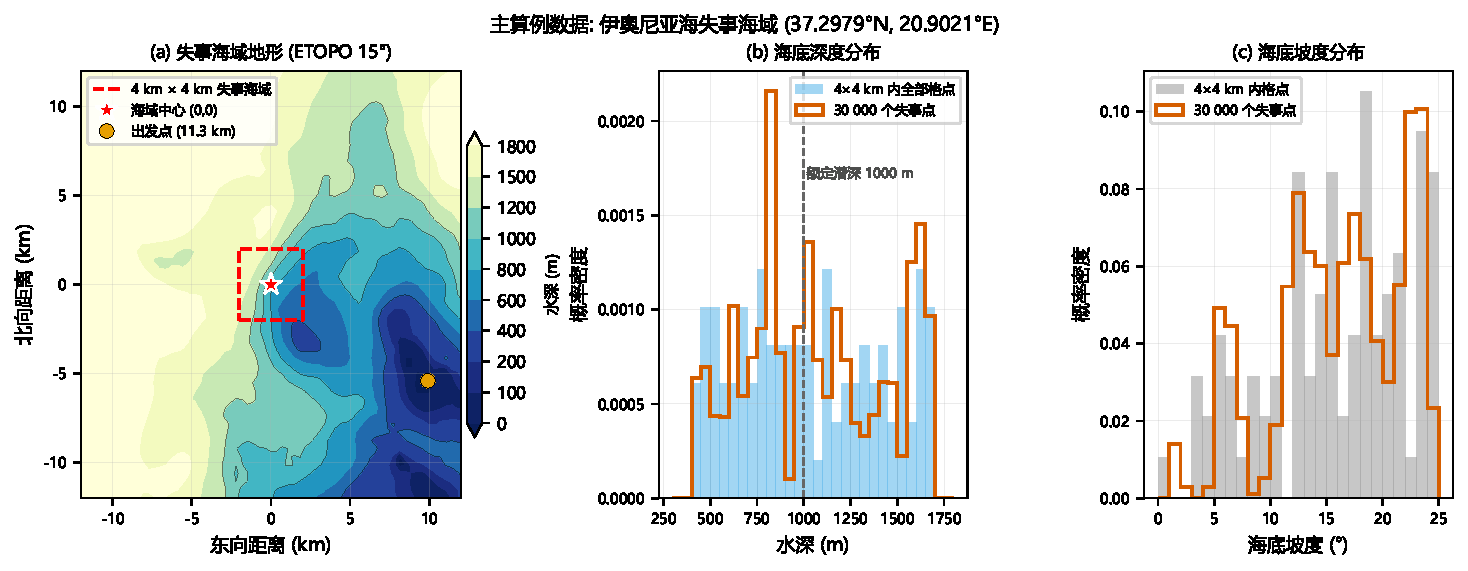
\includegraphics[width=0.82\textwidth]{fig_D1_region}
\caption{主算例海域。(a) 地形与 4$\times$4 km 失事海域、出发点；(b) 海域内海底深度分布
与 30\,000 个失事点的当地海底深度；(c) 海底坡度分布。失事点当地海底深度中位数约
1021 m，坡度中位 16.9°，约 59\% 的点坡度超过 15°。}
\label{fig:region}
\end{figure}

需要说明：4$\times$4 km 海域内约有一半格点水深超过潜水器额定潜深 1000 m。
这不影响失事深度（$z_0\le1000$ m），但会影响沉底分支：若艇体沉到 1000 m 以下的海底，
则认为发生压溃（作为事后统计，见 §\ref{sec:crush}）。这也是“深海沟边缘”海域的重要特征。

\subsection{流场与温盐剖面 (HYCOM GLBy0.08)}

使用 HYCOM GLBy0.08 全球预报产品（水平分辨率约 $0.08^\circ\approx8$ km，
时间分辨率 3 h）。为了支撑 96 h 的漂移模拟，我们下载：

\begin{itemize}[leftmargin=1.8em,itemsep=0pt]
\item \textbf{温盐剖面}：单点 40 层 T/S/u/v，用于计算现场密度、声速与层结；
\item \textbf{四维流场}：17 个时刻（0--96 h，间隔 6 h）$\times$ 6 个深度层
      （0、100、300、500、700、1000 m）$\times$ 20$\times$17 网格，其余深度/时间用线性插值。
\end{itemize}

\begin{figure}[H]
\centering
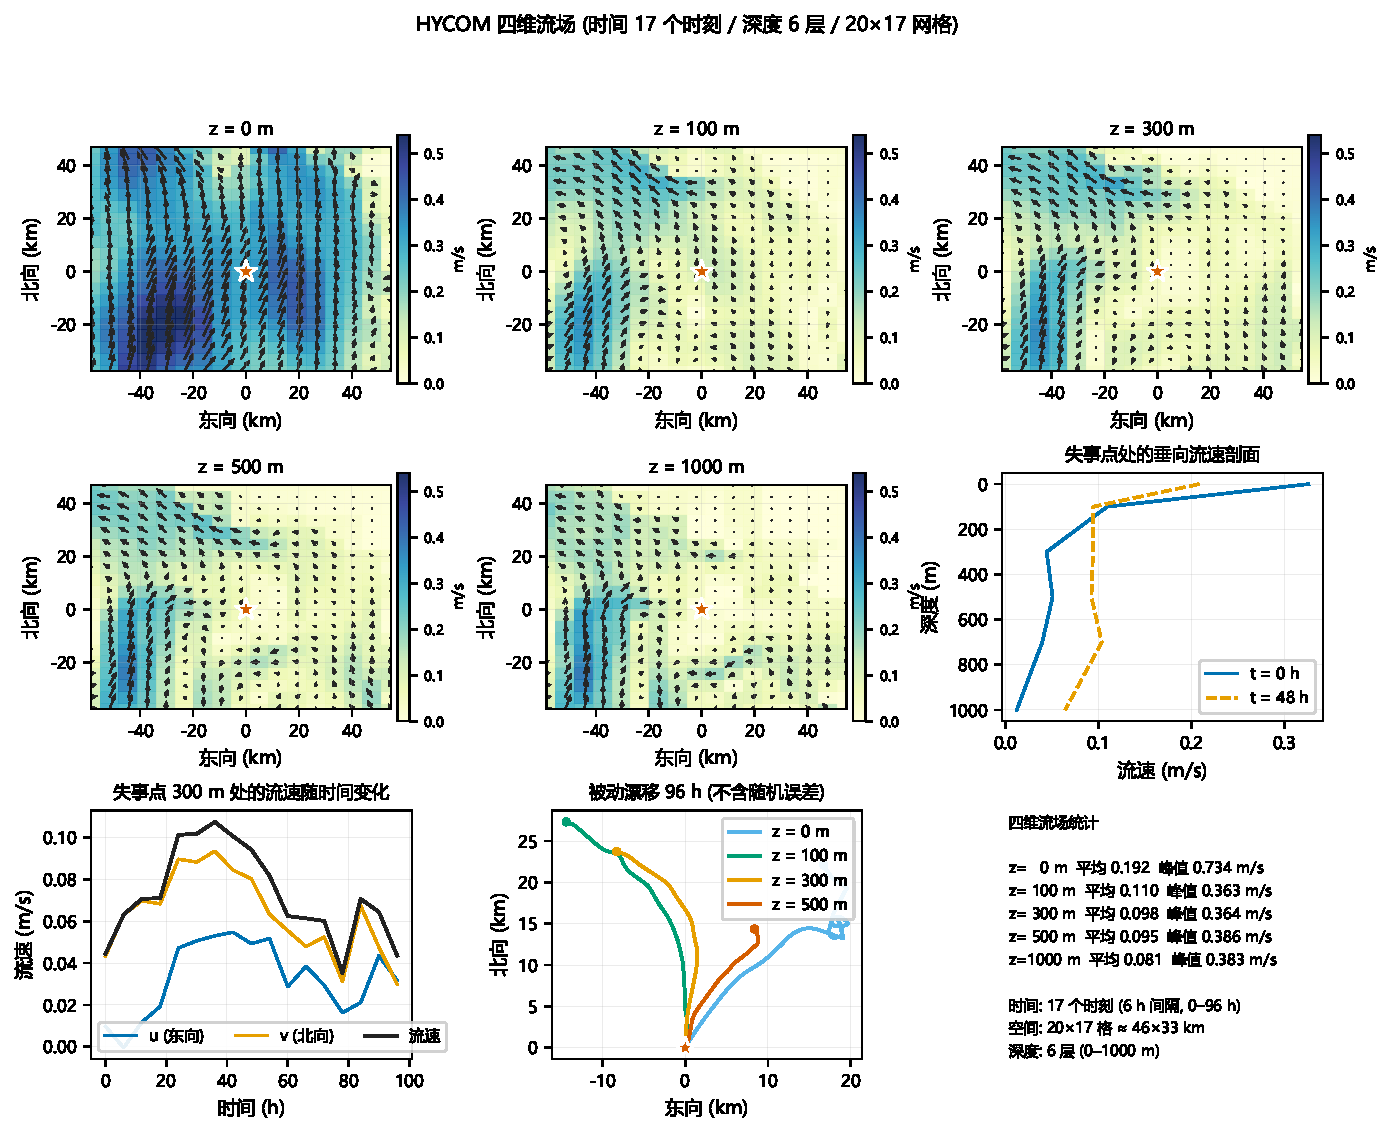
\includegraphics[width=0.66\textwidth]{fig_p2_current}
\caption{HYCOM 四维流场（主算例）。五个深度层（0/100/300/500/1000 m）的流速与流向、
站点垂向流速剖面、300 m 处流速时间序列、以及被动漂移轨迹（不含随机项）。表层流速
平均约 0.19 m/s、峰值 0.73 m/s，100--500 m 层平均约 0.1 m/s。}
\label{fig:current}
\end{figure}

\figref{fig:current} 显示本海域流场是“表层强、深层弱”的结构：0 m 平均流速
0.19 m/s，300 m 以下平均约 0.08--0.10 m/s。这一结构对后面两个结论很关键：
（1）水面分支漂移远、水柱/沉底分支漂移小；（2）搜索装备的水柱能力比“抗漂移”更重要。

\subsection{潜水器参数}

\begin{table}[H]
\centering\small
\caption{潜水器主要参数（Triton 3300/6 厂商数据表）}
\label{tab:vehicle}
\begin{tabular}{@{}ll|l@{}}
\toprule
参数 & 数值 & 说明\\
\midrule
艇体质量 $m$ & 11\,000 kg & 数据表 24,300 lb\\
外形尺寸 & 4.55 m $\times$ 3.60 m $\times$ 2.40 m & 长 $\times$ 宽 $\times$ 高\\
额定潜深 & 1000 m & 3300 ft\\
载员 & 6 人（1 驾驶员 + 5 乘客） & 题设\\
阻力系数 $C_D$ & 0.45 & 球体标准阻力曲线取值\\
附加质量系数 & 0.50 & 球体理论值（Lamb 1932）\\
\bottomrule
\end{tabular}
\end{table}

\subsection{失效模式与先验}

依据“泰坦号”事故链与一般潜水器故障模式，我们把失联后的演化分为 5 种失效模式
（\tabref{tab:failure}）。模式概率由专家判断给出（无公开统计），在报告中作为假设值，
并做敏感性讨论。

\begin{table}[H]
\centering\small
\caption{失效模式树：5 种模式互斥且完备}
\label{tab:failure}
\begin{tabular}{@{}llcl@{}}
\toprule
模式 & 名称 & 概率 & 后续演化\\
\midrule
S0 & 失联但系统正常，自动上浮 & 15\% & 上浮到水面，随表层流与风漂移\\
S1 & 失去推进 + 失联，近中性浮力 & 55\% & 在失事深度附近定深漂流\\
S2 & 断电 & 15\% & 抛载成功（7.5\%）上浮；失败（7.5\%）无动力中性漂流\\
S3 & 耐压壳进水/失效 & 10\% & 快速下沉（$\Delta\rho\approx$20--60 kg/m$^3$）→ 沉底\\
S4 & 压载舱进水 & 5\% & 中速下沉（$\Delta\rho\approx$5--20 kg/m$^3$）→ 沉底\\
\bottomrule
\end{tabular}
\end{table}

\begin{table}[H]
\centering\small
\caption{模型先验分布（全部标注为假设值）}
\label{tab:prior}
\begin{tabular}{@{}lll@{}}
\toprule
参数 & 分布/取值 & 备注\\
\midrule
失事海域 & 4 km $\times$ 4 km 均匀 & 上层给定\\
失事深度 $z_0$ & $p(z)\propto e^{-(z-200)/200}$, $z\ge200$ m & 截断于海底与 1000 m\\
浮力异常 $\Delta\rho$（S1） & $\mathcal N(0,0.05^2)$，截断 $[-0.3,0.3]$ & kg/m$^3$\\
浮力异常（S2b） & $U(0.02,0.5)$ & 同上\\
浮力异常（S3） & $U(20,60)$ & 快速下沉\\
浮力异常（S4） & $U(5,20)$ & 中速下沉\\
静摩擦系数 $\mu_s$ & $U(0.2,0.5)$ & 库仑滑移判据\\
动/静摩擦比 & 0.8 & 经验值\\
阻力系数 $C_D$ & $\mathcal N(0.45,0.05^2)$，截断 $[0.3,0.6]$ & 不确定性\\
OU 流速扰动 & $\sigma=0.03$ m/s，$\tau=3$ h & 中尺度流误差\\
系统偏差 & $\mathcal N(0,0.02^2)$ m/s & 流场整体偏差\\
水平扩散 $K_h$ & 2 m$^2$/s & 湍流随机游走\\
风 & $U(4,12)$ m/s，风阻系数 0.03 & 仅水面分支\\
初始定位误差 & 圆柱 $r=100$ m，$\Delta z=\pm10$ m & 搜救方知识\\
压溃深度 & $1.5\times$ 额定潜深 = 1500 m & 仅事后统计\\
\bottomrule
\end{tabular}
\end{table}

\subsection{数据来源汇总}

\begin{table}[H]
\centering\small
\caption{数据来源、分辨率与用途}
\label{tab:data}
\begin{tabular}{@{}llll@{}}
\toprule
数据 & 来源 & 分辨率 & 用途\\
\midrule
地形 & ETOPO 2022 (NOAA) & $15^{\prime\prime}$ (约 460 m) & 海底深度、坡度、滑移\\
三维流场 & HYCOM GLBy0.08 & $\sim$8 km / 3 h / 40 层 & 四维插值漂移\\
温盐剖面 & HYCOM GLBy0.08 & 站点 40 层 & 密度、声速、层结\\
艇体参数 & Triton 3300/6 数据表 & — & 质量、尺寸、阻力\\
失效概率 & 专家判断（假设） & — & 模式先验\\
装备参数 & 公开市场量级估计 & — & 扫宽、速度、成本\\
\bottomrule
\end{tabular}
\end{table}
